% Partie training (Noé Mosca) : perte relativiste, R1 et EMA.
% Chiffres : enquete/results/juliet/juliet2_test.csv (BCE brut / EMA, A100), results/comparison_local.csv (baseline Mac, RpGAN + EMA),
% enquete/results/ema/ema_summary.csv (RpGAN brut), kid_perclass_all.csv (FID par chiffre), enquete/training.md (balayage gamma,
% effondrements, équilibre de D), PLAN.md §2 (réplication A100). Figure : figscripts/training.py -> figures/training_perdigit.pdf.
\section{Training: relativistic loss, R1 and EMA}\label{sec:training}

\textbf{Hypotheses.} H1: the sigmoid BCE saturates (collapse) and drifts to easy digits; a relativistic loss with R1 keeps $G$'s gradient informative. H2: averaging $G$'s weights removes the oscillation around equilibrium.

\textbf{Method.} $D(x)$: raw score of $D$ (before the sigmoid); $\mathrm{sp}(t)=\log(1+e^t)$. RpGAN~\cite{jolicoeur2019} scores a pair (real $x$, fake $\tilde x$); R1~\cite{mescheder2018} penalises $D$'s slope on real images (we omit R2, its fake-image twin in R3GAN~\cite{huang2024}):
\begin{align*}
L_D &= \mathrm{sp}\big(D(\tilde x)-D(x)\big) + \tfrac{\gamma}{2}\,\|\nabla_x D(x)\|^2,\\
L_G &= \mathrm{sp}\big(D(x)-D(\tilde x)\big).
\end{align*}
EMA~\cite{yazici2019}: after each step, $G_\mathrm{EMA}\leftarrow\beta\,G_\mathrm{EMA}+(1-\beta)\,G$, $\beta=0.999$ (half-life $\approx$\,1.4 epochs). Training uses only raw $G$: each run yields both, so EMA effects are paired.

\begin{figure}[t]
\centering
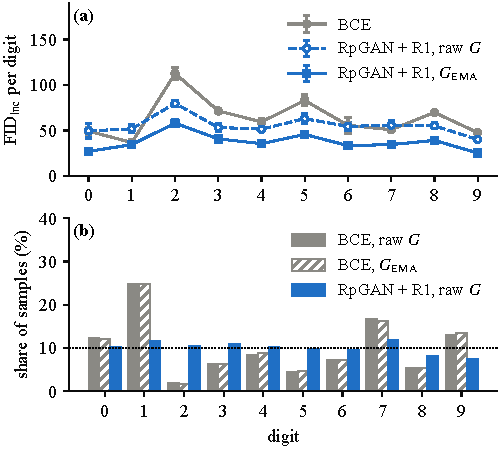
\includegraphics[width=\columnwidth]{training_perdigit}
\caption{\textbf{RpGAN + R1 fixes the digit mix; EMA cleans every digit.} Common protocol, 3 seeds. (a) Per-digit FID$_\text{Inc}$ (real data: 6.5--10.4). (b) Share of each digit in 10\,000 samples (dotted: 10\%). BCE: Mac in (a), cluster in (b).}
\label{fig:training-perdigit}
\end{figure}

\begin{table}[t]
\centering\footnotesize\setlength{\tabcolsep}{3pt}
\caption{\textbf{Loss $\times$ EMA} (common protocol).}
\label{tab:training-ema}
\begin{tabular}{@{}llcccc@{}}
\toprule
 & & \multicolumn{2}{c}{BCE} & RpGAN + R1 & Loss $\Delta$\\
\cmidrule(lr){3-4}
 & & Mac & cluster & Mac & ($p$)\\
\midrule
raw $G$ & FID$_\text{Inc}$ & 38.7$\pm$1.2 & 36.6$\pm$1.3 & 37.7$\pm$1.0 & $-1.0$ (0.35)\\
 & P/R & 0.47/0.51 & 0.48/0.49 & 0.47/0.47 & \\
$G_\mathrm{EMA}$ & FID$_\text{Inc}$ & -- & 30.0$\pm$0.2 & \textbf{22.1}$\pm$1.3 & $-7.8$ (0.007)\\
 & P/R & -- & 0.56/0.54 & 0.59/0.59 & \\
\midrule
\multicolumn{2}{@{}l}{EMA $\Delta$ ($p$)} & -- & $-6.7$ (0.01) & $-15.6$ (${<}0.001$) & \\
\bottomrule
\end{tabular}
\tabnote{P/R: VGG. EMA $\Delta$: paired $t$; loss $\Delta$: Welch vs BCE (cluster for $G_\mathrm{EMA}$, Mac for raw $G$). EMA $\Delta$ on RpGAN: both $G$ re-scored on the cluster.}
\end{table}

\subsection{RpGAN + R1 (H1)}
\textbf{Expected.} A large gain if the baseline is unstable, a small one otherwise (CIFAR-10~\cite{jolicoeur2019}). R3GAN: RpGAN + R1 \emph{fails} on StackedMNIST without R2~\cite{huang2024}.

\textbf{Observed.} \emph{$\gamma$ sweep} (FID$_\text{CNN}$; protocol in Table~\ref{tab:intro-protocol}): $\gamma=0.1$ diverges (3/3), $\gamma=1$ is best ($14.0\pm0.9$), $\gamma=10$ worse ($17.7\pm0.9$, still falling at 100 epochs); adding R2 changes nothing ($14.4\pm0.9$). $\gamma\ge1$ never collapsed (0/12: 9 sweep + 3 common runs; BCE: 1/3 in the sweep, Fisher $p=0.20$; 0/6 common).
\emph{Common protocol, raw $G$:} FID$_\text{Inc}$ is flat (Table~\ref{tab:training-ema}), but the mix is fixed (Fig.~\ref{fig:training-perdigit}b; FID$_\text{CNN}$ $182\to19.7$) and strokes improve at fixed digit (per-digit FID$_\text{Inc}$ $63.6\to55.4$, $p=0.005$), most on ``2'' (113 $\to$ 80); ``1'' and ``7'' worsen.

\textbf{Why.} Within RpGAN, R1 is needed against collapse: without it, $D$ wins within 1--2 epochs (1 seed); with $\gamma=0.1$, 3/3 seeds diverge before epoch 10. Whether R1 suffices with the BCE is untested. Unpenalised, $G$ and $D$ circle around equilibrium; R1 damps this (hypothesis: in Mescheder's toy GAN, one parameter each for $G$ and $D$~\cite{mescheder2018}, circling stops at $\gamma=1$ for our loss, our best grid point). The pooled FID$_\text{Inc}$ hides the stroke gain: the BCE rarely draws its worst digit.

\textbf{When it fails.} $\gamma\le0.1$. Unlike R3GAN we need no R2: likely an easier task (10 modes), small networks, Adam $\beta_1=0.9$ not 0 (with theirs our run collapses, 1 seed).

\subsection{EMA, and why the gain needs both (H2)}
\textbf{Expected.} EMA cuts FID by 24--29\% on CIFAR-10~\cite{yazici2019}.

\textbf{Observed} (Table~\ref{tab:training-ema}). The EMA gain doubles from the BCE ($-6.7$, $-18\%$) to RpGAN + R1 ($-15.6$, $-41\%$; interaction $p=0.002$); P and R rise together: no trade-off. The loss gives $-7.8$ with EMA (BCE + EMA on the cluster, which favours it), nothing detectable without (a cluster rerun, best checkpoint, agrees: 36.4 vs 36.1). On RpGAN + R1, EMA improves every digit ($55.4\to37.3$, 30/30 \mbox{seed--digit} pairs; Fig.~\ref{fig:training-perdigit}a); on the BCE it leaves the mix unfixed (FID$_\text{CNN}$ $170\to182$, n.s.).

\textbf{Why (hypothesis).} At the end, RpGAN's $D$ barely separates real from fake (mean $\sigma(D)$ 0.62 vs 0.59; BCE 0.72 vs 0.28): $G$ oscillates near equilibrium, and the average lands near its centre~\cite{yazici2019}. The BCE drifts instead (validation FID$_\text{CNN}$: best 50--65 at epochs 100--120, 159--196 at epoch 200); a 1.4-epoch average cannot undo a drift.

\takeaway{RpGAN + R1 fixes the digit mix (no collapse with $\gamma\ge1$, 0/12; n.s.\ vs BCE); EMA cleans every digit; the loss pays off only with EMA.}
